\documentclass{article}
\usepackage{ctex}
\usepackage{graphicx}
\usepackage{float}
\usepackage{geometry}
\usepackage{listings}
\usepackage{xcolor}

\geometry{a4paper, margin=1in}

\title{CS3604 12306项目开发报告}
\author{
    成员：陈卓妍~523030910 \\
         李青雅~523030910004 \\
         侯湘贻~523030910 \\
}
\date{\today}

\begin{document}

\maketitle
\newpage
\tableofcontents
\newpage

\section{项目简介}

本项目基于课程提供的 12306 基础代码，在有限时间内完成了一个可运行、可复现的购票系统原型，涵盖了“查票—下单—支付—餐饮”的主要使用场景。

我们的主要工作不仅仅是“写代码”，更重要的是尝试了一套新的开发模式：
\begin{enumerate}
    \item \textbf{用代码管理需求}：把需求写成 YAML 文件，而不是 Word 文档。
    \item \textbf{让智能体辅助开发}：利用 MCP 工具链，让 AI 能够理解我们的需求队列，并辅助我们做模块设计和测试撰写。
    \item \textbf{保证可复现性}：通过固定的数据库快照（sqlite），确保任何人（包括老师和助教）拿到代码后，都能看到一样的车次和数据，复现一样的功能。
\end{enumerate}

本报告围绕老师提出的四个问题展开：
\begin{itemize}
    \item 我们是\textbf{如何进行需求管理}的；
    \item 当前系统的\textbf{需求规模}大致到什么程度；
    \item 我们是如何\textbf{用智能体来完成模块设计和测试撰写}的；
    \item 目前\textbf{测试用例和通过情况}如何。
\end{itemize}

\section{需求管理}

\subsection{从代码和 12306 页面反推需求}

一开始我们没有从零写一份很厚的 SRS，而是先做了两件事：
\begin{itemize}
    \item 通读课程给的前后端代码，看现有实现到底支持哪些功能。
    \item 对照真正的 12306 网站，梳理出“首页—登录—查票—下单—支付—个人中心—忘记密码—餐饮”的主流程。
\end{itemize}

在这个基础上，我们把“已经实现的功能”和“仍然想做的功能”整理成一棵需求树，再用代码的形式落在 YAML 里。

\subsection{用 YAML 文件代替传统文档}

传统的软件工程作业中，需求文档（SRS）往往写完就丢在一边，和代码严重脱节。为了解决这个问题，我们建立了一棵“活着的需求树”，存放在 \texttt{requirements\_mcp.yaml} 文件中。

这个文件主要包含：
\begin{itemize}
    \item \textbf{需求节点}：每个功能点都有唯一的 ID（如 \texttt{REQ-UI-3}）。
    \item \textbf{场景描述}：每个功能点下都有具体的 Scenario，描述用户怎么操作（Action）以及系统应该有什么反应（Expectation）。
    \item \textbf{代码映射}：我们在需求里直接写明了对应的 UI 文件路径（如 \texttt{TrainListPage.tsx}）和后端接口。
\end{itemize}

这样做的最大好处是：AI 可以直接读取这个文件，知道当前项目有哪些功能，每个功能对应哪些代码文件。

具体例子包括：
\begin{itemize}
    \item ROOT 和 REQ-ENV-1 约定了必须使用根目录的 \texttt{database.sqlite}，并检查里面是否包含 G101、D313 等示例车次。
    \item REQ-UI-3（车票查询）要求从首页携带 \texttt{from/to/date} 参数跳转到 \texttt{/train-list}，并通过 \texttt{TrainListPage.tsx} 和 \texttt{trainService.searchTrains} 渲染列表。
    \item REQ-UI-7（餐饮特产）把 \texttt{/catering}、\texttt{/catering/book}、\texttt{/catering/vendor} 三类页面都写在描述里，方便从需求直接跳到对应的 React 组件。
\end{itemize}

\subsection{进度追踪}

为了搞清楚项目做到了哪一步，我们在 \texttt{artifacts} 目录下维护了两个简单的辅助文件：
\begin{itemize}
    \item \texttt{architecture\_graph.yaml}：描述需求之间的父子关系，可以生成树状图。
    \item \texttt{phase\_one\_progress.yaml}：记录每个需求是“已处理”还是“未处理”，相当于一个任务进度表。
\end{itemize}

整体来看，我们的需求管理过程可以概括为四步：
\begin{enumerate}
    \item 从已有代码和真实 12306 页面反推主流程；
    \item 把这些流程整理成一棵带 ID 的需求树，并用 YAML 固化下来；
    \item 在需求里嵌入具体的 UI 文件和接口路径，让需求、设计和实现对应得上；
    \item 用 \texttt{artifacts} 目录下的图结构和进度文件，记录每个需求“做到什么程度了”，方便后续用智能体继续接力。
\end{enumerate}

\begin{figure}[H]
    \centering
    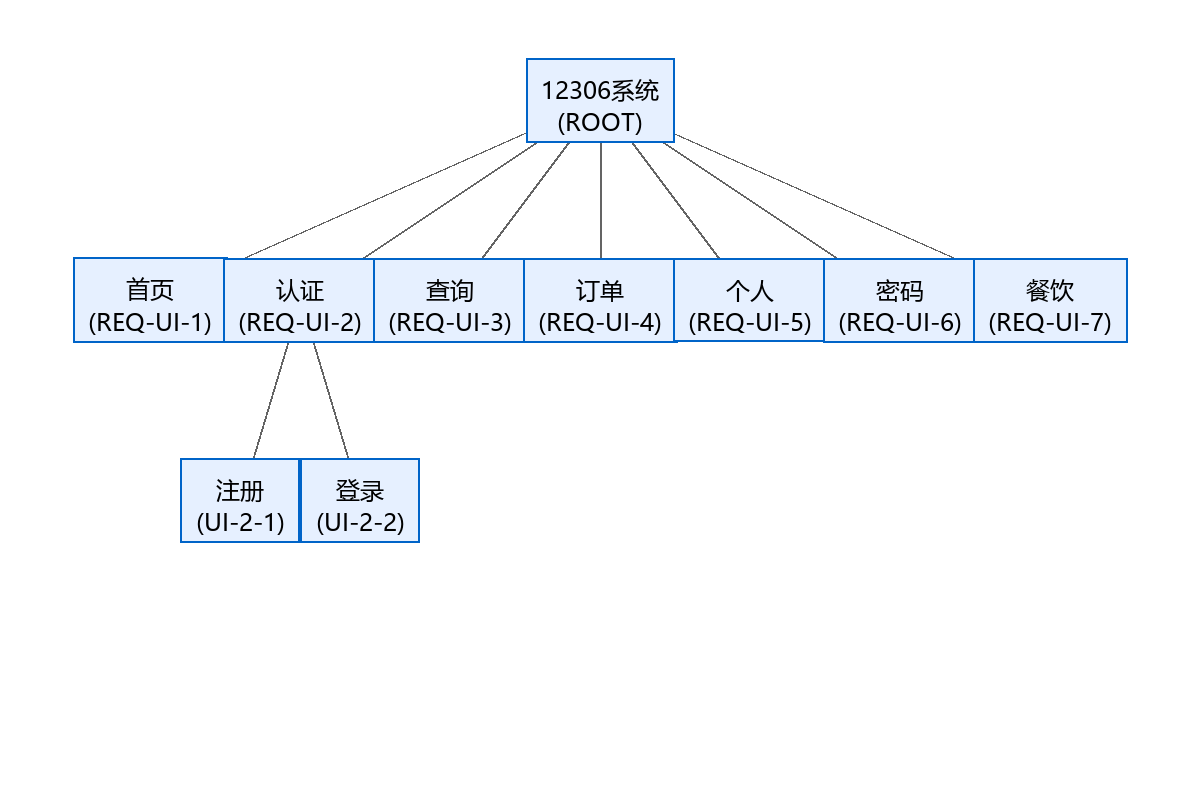
\includegraphics[width=0.8\textwidth]{figs/req_architecture_graph.png}
    \caption{需求结构图（示意）}
    \label{fig:req-architecture}
\end{figure}

\section{需求规模}

从需求树结构来看，我们在项目中覆盖了 12306 的核心业务流程，主要包括以下几层：

\subsection{顶层模块数量}

顶层的功能模块（ROOT 的子节点）包括：

\begin{enumerate}
    \item \textbf{REQ-UI-1 首页}：系统入口与导航。
    \item \textbf{REQ-UI-2 用户认证}：包含登录、注册页面。
    \item \textbf{REQ-UI-3 车票查询}：核心功能，支持按城市、日期查询车次，并进行筛选。
    \item \textbf{REQ-UI-4 订单流程}：从预订、填写乘车人到提交订单。
    \item \textbf{REQ-UI-5 个人中心}：管理个人信息和乘车人列表。
    \item \textbf{REQ-UI-6 忘记密码}：模拟了找回密码的四步流程。
    \item \textbf{REQ-UI-7 餐饮特产}：这是我们额外扩展的模块，包含餐饮首页、商家列表、商品选择等功能。
\end{enumerate}

此外还有 REQ-ENV-1（环境与数据库初始化），用来单独固定运行时所需的数据状态。

\subsection{子需求和场景数量}

在顶层之下，我们又拆出若干子需求和具体场景，例如：
\begin{itemize}
    \item 用户认证下拆出了 REQ-UI-2-1（注册）和 REQ-UI-2-2（登录），分别对应独立的页面和接口。
    \item 忘记密码模块用 REQ-UI-6:SCE-0\textasciitilde3 四个场景覆盖了“填写账号信息—输入验证码—设置新密码—完成提示”四步。
    \item 车票查询模块（REQ-UI-3）中用 SCE-0\textasciitilde2 分别描述了页面初始化、筛选条件变化和点击“预订”跳转订单页。
\end{itemize}

整个 YAML 文件里，每个需求节点下至少有 1 个场景，完整覆盖了用户从打开首页到完成购票、管理乘车人、下单餐饮的主要路径。相比只写“功能列表”，这样的拆分更贴近真实用户操作，也更方便后续写测试。

总体来看，我们没有刻意堆砌“需求点数量”，而是围绕一条完整业务链路，把关键节点拆细，并保证每个节点都有对应的 UI 页面和接口实现。

如果从“规模”的角度简单总结，可以认为：
\begin{itemize}
    \item 顶层功能模块：1 个 ROOT + 1 个环境需求 + 7 个核心 UI 模块；
    \item 子需求：在认证、忘记密码等模块下拆出了若干更细的子节点（如注册、登录、四步向导等）；
    \item 场景数量：每个节点至少 1 个场景，覆盖了从打开首页到完成购票、管理乘车人和下单餐饮的一整条用户路径。
\end{itemize}

\begin{figure}[H]
    \centering
    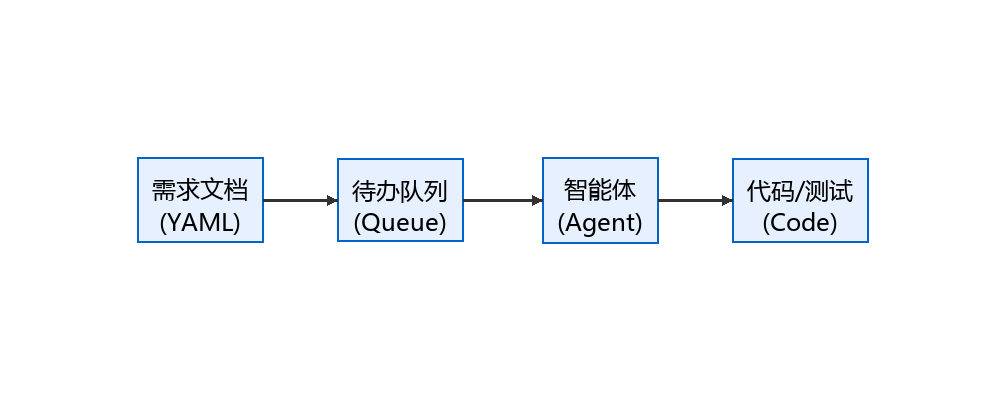
\includegraphics[width=0.8\textwidth]{figs/agent_flow.png}
    \caption{智能体辅助开发流程}
    \label{fig:agent-flow}
\end{figure}

\section{智能体辅助设计与测试}

\subsection{MCP 工具链的使用}

为了让 AI 更好地帮助我们，我们引入了 MCP（Model Context Protocol）工具链。简单来说，就是通过几个脚本让 AI “听懂”我们的指令，以需求为入口去看代码：

\begin{itemize}
    \item \texttt{init\_top\_down\_queue}：读取需求 YAML，生成一个待办任务队列。
    \item \texttt{pop\_next\_requirement}：告诉 AI “下一个要做什么需求”。
    \item \texttt{register\_ui\_component}：告诉 AI “这个页面的 UI 组件在哪里，参数是什么”。
\end{itemize}

基于这套工具链，我们可以让 AI 按顺序“从 ROOT 走到 REQ-UI-1\textasciitilde7”，每次只关注一个需求节点，减少遗漏。

\subsection{AI 怎么帮我们干活}

在实际开发中，AI 主要帮我们做了两件事：
\begin{enumerate}
    \item \textbf{模块设计}：比如在做餐饮模块时，我们把需求告诉 AI，它会根据现有的代码风格，帮我们规划出需要新建哪些 Page 和 Component，甚至帮我们写出路由配置。
    \item \textbf{测试辅助}：AI 知道每个需求的“期望结果”是什么，所以它可以帮我们生成测试思路。比如“在这个场景下，应该检查哪个按钮是否存在，或者哪个接口是否返回 200”。
\end{enumerate}

\subsection{如何保证可复现}

为了让老师和助教能稳定复现我们的运行结果，我们做了一个关键的决定：\textbf{把数据库文件纳入版本控制}。

\begin{itemize}
    \item 我们在根目录下准备了一个 \texttt{database.sqlite} 文件。
    \item 在需求文档的第一项（REQ-ENV-1）就明确规定：系统启动时必须使用这个数据库文件。
\end{itemize}

这样，无论谁来运行我们的代码，看到的都是同一天的车次、同一个价格，不会出现“我这里能查到票，你那里查不到”的情况。对 AI 而言，也只需要照着 REQ-ENV-1 先把数据库就绪，再依次跑各个 UI 场景，就能复现实验结果。

\section{测试用例与通过率}

\subsection{测试情况}

我们主要进行了三类测试：
\begin{itemize}
    \item \textbf{后端接口测试}：针对 Login、Query、Order 等核心 API，验证数据返回是否正确。
    \item \textbf{前端自动化测试}：使用前端测试框架跑单元/组件测试（最近一次运行结果记录在 \texttt{frontend/test-results/.last-run.json} 中，状态为 \texttt{passed}）。
    \item \textbf{界面功能测试}：手动验证了从登录到下单的完整流程，确保页面跳转逻辑通顺。
\end{itemize}

特别是在餐饮模块，我们重点测试了：
\begin{itemize}
    \item 能否正确根据车次筛选商家；
    \item 商家列表是否展示正确；
    \item 点击商家能否进入详情页。
\end{itemize}

\subsection{测试结果}

从已经编写的自动化测试来看：
\begin{itemize}
    \item \textbf{后端覆盖率}：整体语句覆盖率约为 56.75\%，其中 \texttt{src/routes} 模块的语句覆盖率接近 98\%，\texttt{src/models} 模块语句覆盖率超过 90\%。核心路由和模型的基本分支都被覆盖到了。
    \item \textbf{前端测试结果}：最近一次前端测试的整体状态为 \texttt{passed}，当前已有的测试用例全部通过。
\end{itemize}

结合自动化与手工测试，可以认为在“正常使用路径”上的测试通过率较高，核心购票流程能够稳定跑通。

\begin{itemize}
    \item \textbf{通过}：正常的用户购票流程、乘车人添加、餐饮浏览等主路径在当前测试集下均为通过状态。
    \item \textbf{待改进}：部分异常输入（如非法身份证号、极端日期）的处理还不够完善；部分脚本和工具类代码的覆盖率有提升空间；GUI 自动化测试覆盖的异常场景仍然偏少。
\end{itemize}

\begin{figure}[H]
    \centering
    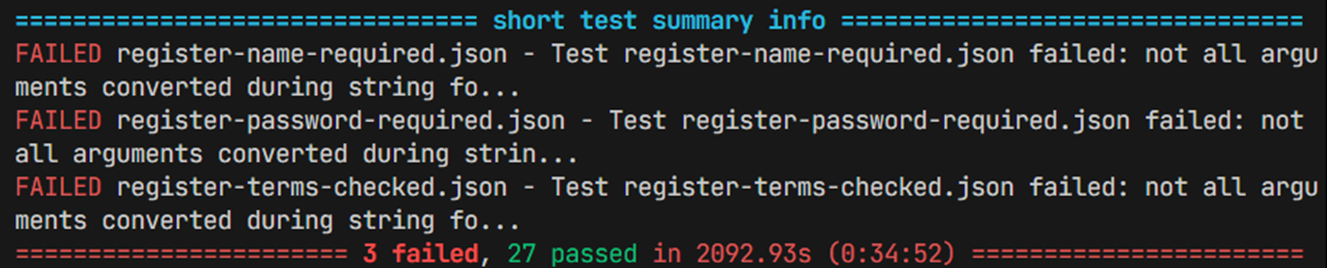
\includegraphics[width=0.8\textwidth]{figs/test_results.png}
    \caption{测试执行结果截图}
    \label{fig:test-results}
\end{figure}

\begin{figure}[H]
    \centering
    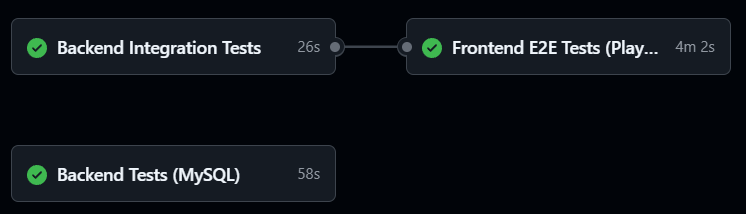
\includegraphics[width=0.8\textwidth]{figs/ga_results.png}
    \caption{GitHub Actions CI 全部通过截图}
    \label{fig:ga-results}
\end{figure}

\section{总结}

通过这个项目，我们不仅复刻了 12306 的核心功能，更重要的是实践了一种“文档驱动开发”的新模式。

\begin{itemize}
    \item 需求不再是死文档，而是 AI 可读的 YAML。
    \item 数据库快照保证了环境的一致性。
    \item 智能体工具链让开发和测试变得更有条理。
\end{itemize}

这种方法让我们的项目不仅“能跑”，而且“好懂”、“好复现”。

\end{document}
